\documentclass[12pt, psamsfonts]{amsart}

%-------Packages---------
\usepackage{amssymb,amsfonts}
\usepackage{fullpage}
\usepackage{tikz-cd}
\usepackage{todonotes}
\usepackage{physics}
\usepackage[all,arc]{xy}
\usepackage{enumerate}
\usepackage{enumitem}
\usepackage{mathrsfs}
\usepackage{theoremref}
\usepackage{graphicx}
\usepackage[bookmarks]{hyperref}

%--------Theorem Environments--------
%theoremstyle{plain} --- default
\newtheorem{thm}{Theorem}[section]
\newtheorem{cor}[thm]{Corollary}
\newtheorem{prop}[thm]{Proposition}
\newtheorem{lem}[thm]{Lemma}
\newtheorem{conj}[thm]{Conjecture}
\newtheorem{quest}[thm]{Question}

\theoremstyle{definition}
\newtheorem{defn}[thm]{Definition}
\newtheorem{defns}[thm]{Definitions}
\newtheorem{con}[thm]{Construction}
\newtheorem{exmp}[thm]{Example}
\newtheorem{exmps}[thm]{Examples}
\newtheorem{notn}[thm]{Notation}
\newtheorem{notns}[thm]{Notations}
\newtheorem{addm}[thm]{Addendum}
\newtheorem*{exer}{Exercise}

\theoremstyle{remark}
\newtheorem{rem}[thm]{Remark}
\newtheorem{rems}[thm]{Remarks}
\newtheorem{warn}[thm]{Warning}
\newtheorem{sch}[thm]{Scholium}

\DeclareMathOperator{\Hom}{Hom}
\DeclareMathOperator{\Id}{Id}
\DeclareMathOperator{\End}{End}
\DeclareMathOperator{\ord}{ord}

\makeatletter
\let\c@equation\c@thm
\makeatother
\numberwithin{equation}{section}

\bibliographystyle{plain}

\begin{document}

\title{Math 611 (Due 10/23)}
\author{Hidenori Shinohara}
\maketitle

\section{Simplicial and Singular Homology}

\begin{exer}{(Problem 2)}
  Show that the $\Delta$-complex obtained from $\Delta^3$ by performing the edge identifications $[v_0, v_1] \sim [v_1, v_3]$ and $[v_0, v_2] \sim [v_2, v_3]$ deformation retracts onto a Klein bottle.
  Find other pairs of identifications of edges that produce $\Delta$-complexes deformation retracting onto a torus, a 2-sphere, and $\mathbb{R}\mathbf{P}^2$.
\end{exer}

\begin{proof}
  The deformation retraction of $\Delta^3$ onto a Klein bottle is described in \ref{fig:problem2_klein_bottle}.
  We will start by ``pushing" $\Delta^3$ from edge $(v_1, v_2)$.
  This will leave the surface that consists of the triangles $[v_0, v_1, v_3]$ and $[v_0, v_2, v_3]$.
  (In other words, a diamond shape consisting of the vertices $[v_0, v_1, v_3, v_2]$.)
  Step 2 in Figure \ref{fig:problem2_klein_bottle} is what $\Delta^3$ should look like after the deformation retract.
  Step 3 through 6 show why this is a Klein bottle.

  \begin{figure}
    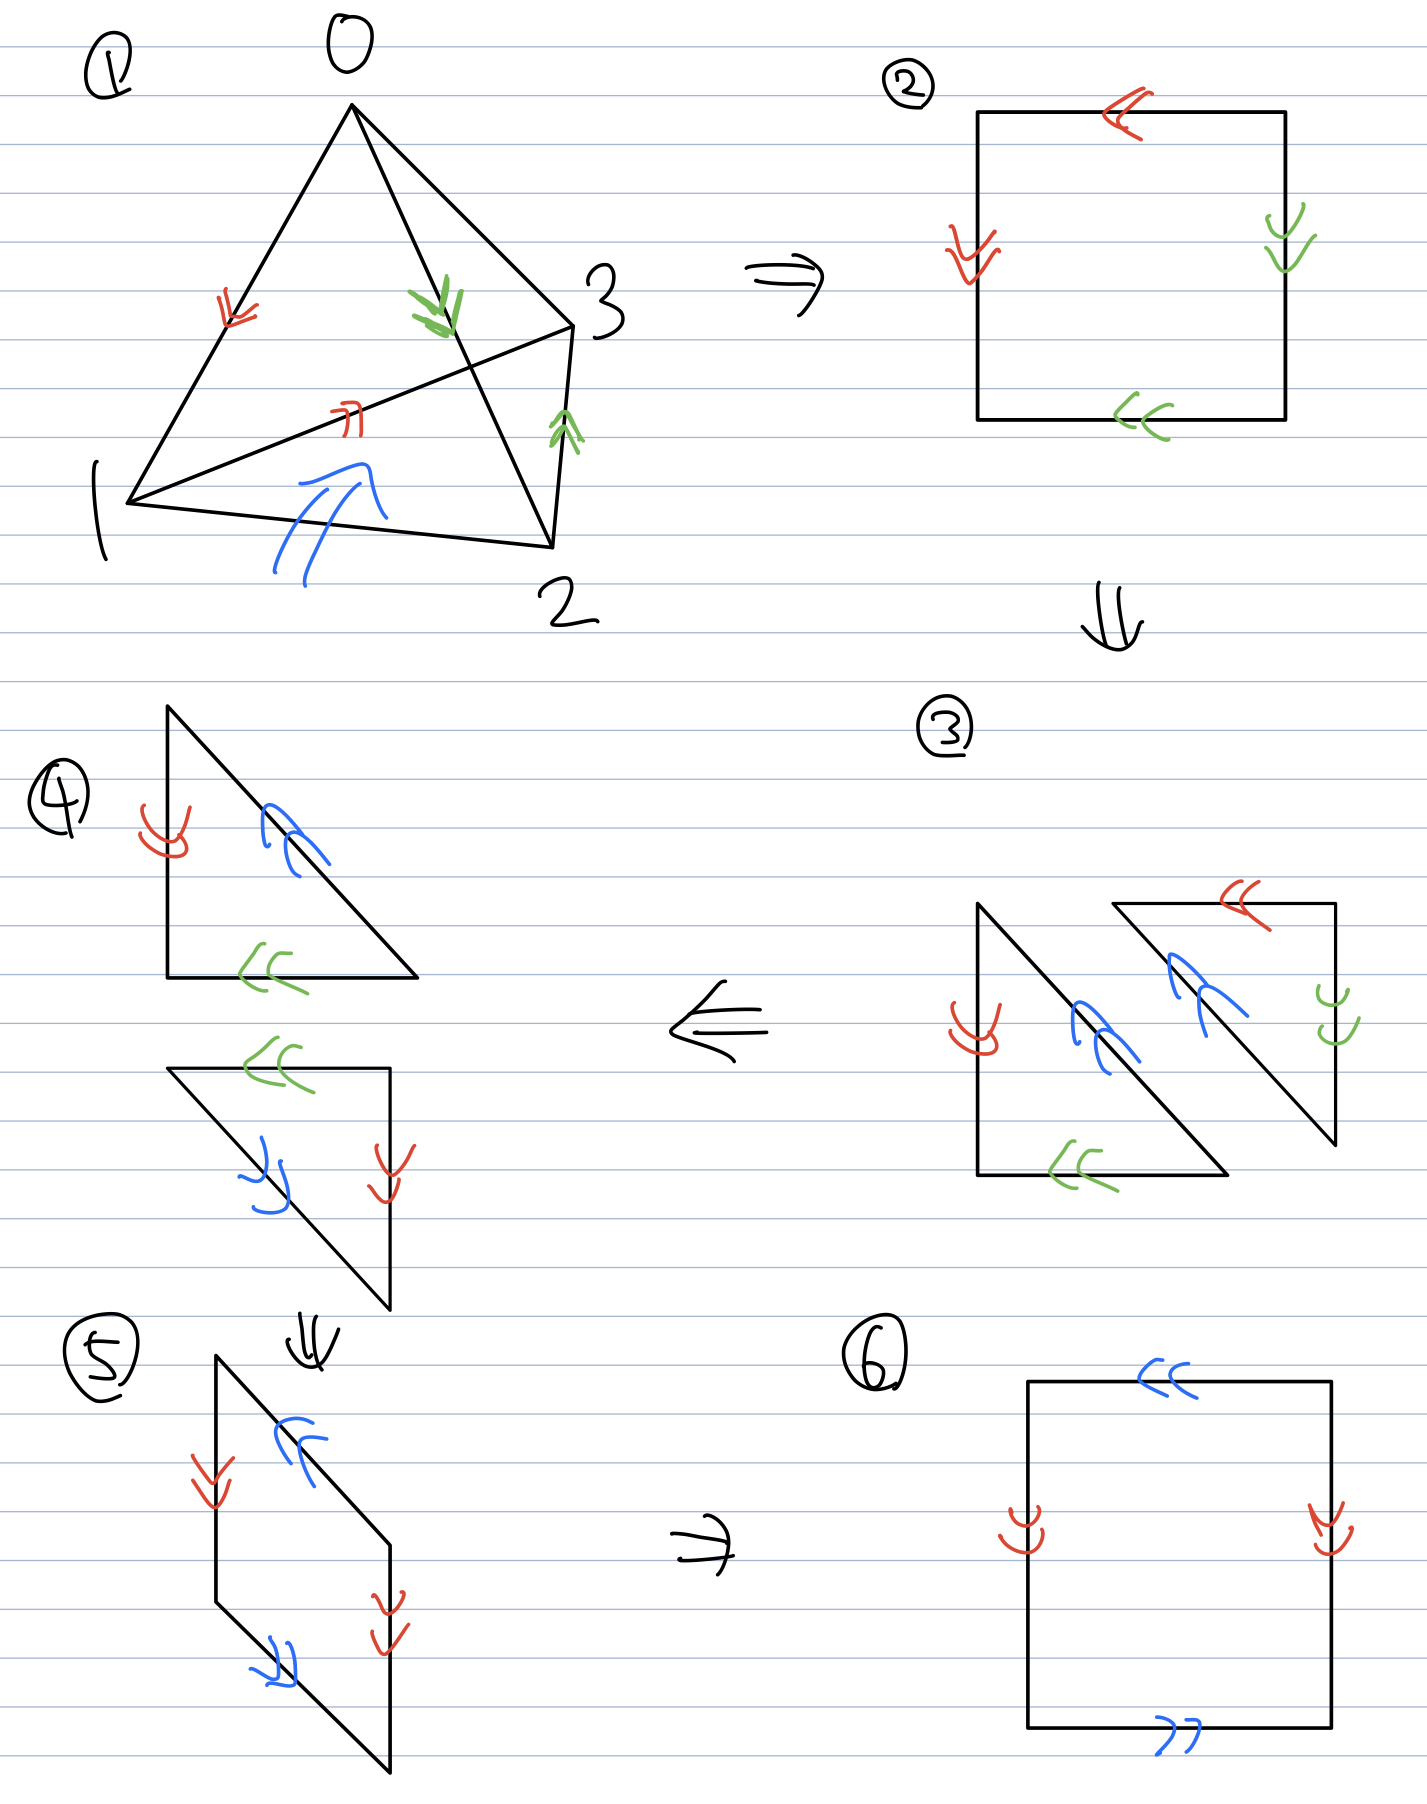
\includegraphics[width=.5\linewidth]{problem2_klein_bottle.jpeg}
    \caption{Problem 2(Klein Bottle)}
    \label{fig:problem2_klein_bottle}
  \end{figure}

  Figure \ref{fig:problem2_torus_sphere_rp2} shows the identification of edges for a torus, 2-sphere, and $\mathbb{R}\mathbf{P}^2$.

  \begin{figure}
    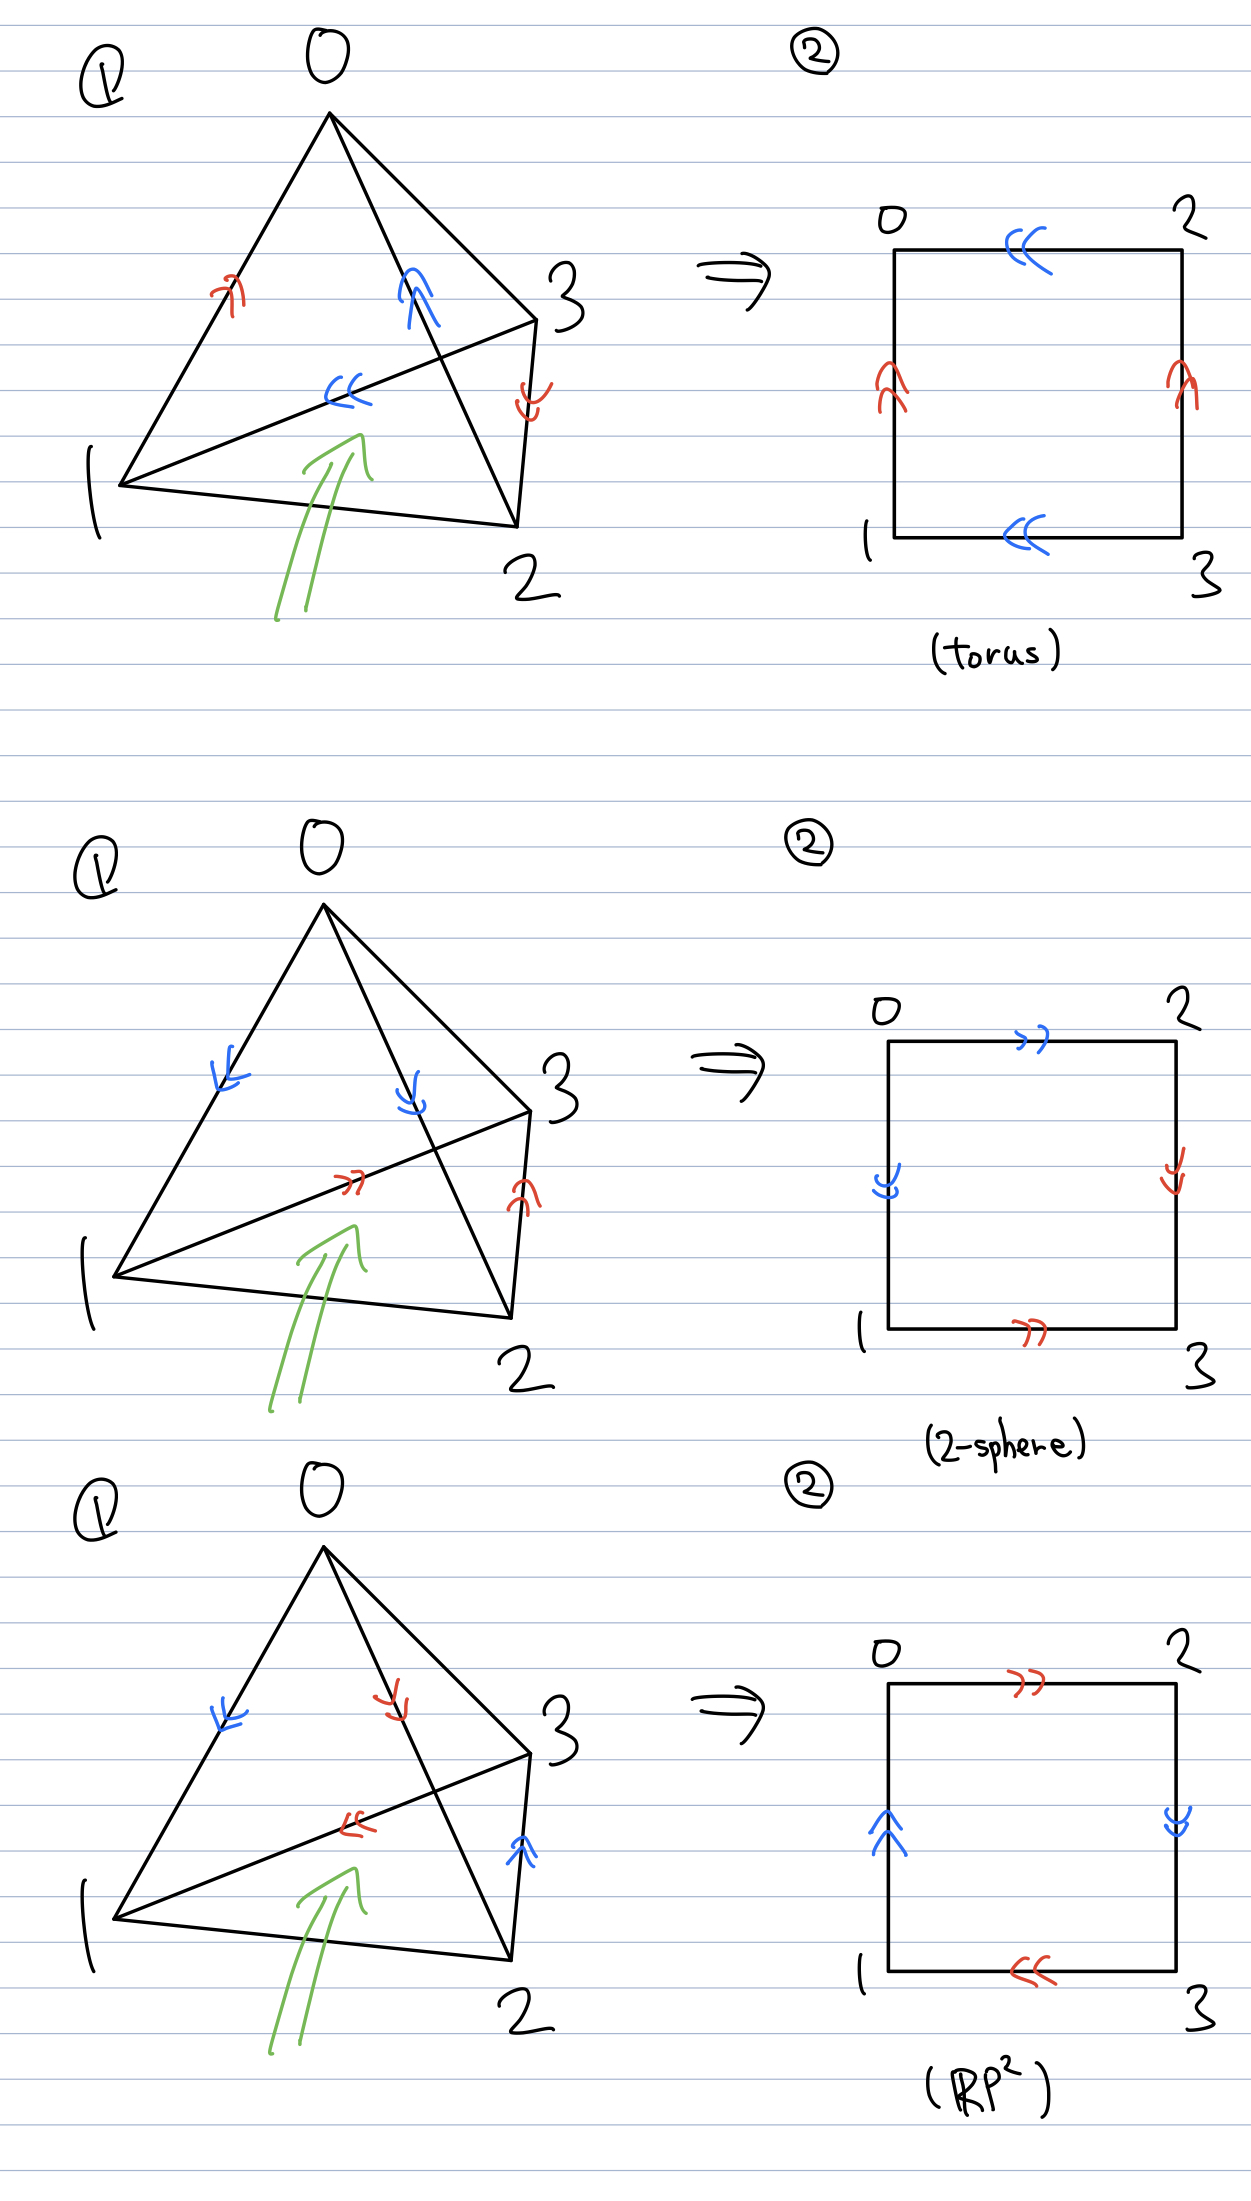
\includegraphics[width=.5\linewidth]{problem2_torus_sphere_rp2.jpeg}
    \caption{Problem 2(Torus, 2-Sphere, $\mathbb{R}\mathbf{P}^2$)}
    \label{fig:problem2_torus_sphere_rp2}
  \end{figure}

\end{proof}

\begin{exer}{(Problem 4)}
  Compute the simplicial homology groups of the triangular parachute obtained from $\Delta^2$ by identifying its three vertices to a single point.
\end{exer}

\begin{proof}
  Let $v_0$ denote the only vertex, $e_1, e_2, e_3$ denote the three edges of the parachute, and $\sigma$ denote the face of the parachute.
  $C_k = 0$ for $k \geq 3$ because $\Delta^2$ with the vertices identified does not contain any $k$-dimensional simplicies.
  $C_2 = \ev{ \sigma}, C_1 = \ev{ e_1, e_2, e_3 }, C_0 = \ev{ v_0 }$.
  Let $n \in \mathbb{N}$.
  $\partial_n$ is defined such that $\partial_n(\sigma_{\alpha}) = \sum_{i}(-1)^i\sigma_{\alpha}\vert[v_0, \cdots, \hat{v_i}, \cdots, v_n]$.
  Since there is only one vertex, $\partial_n$ is the zero map.
  \todo[inline,caption={}]{
    This argument doesn't work.
    Check the torus example from class.
    It only has one vertex, but $\partial_n$ is not the zero map for some $n$.
  }
  Therefore, $H_n = \ker(\partial_n) / \Im(\partial_{n + 1}) = C_n / \ev{ 0 } = C_n$.
  Thus
  \begin{align*}
    H_n &= \begin{cases}
      \{ 0 \} & (n \geq 3) \\
      \ev{ \sigma } \cong \mathbb{Z} & (n = 2) \\
      \ev{ e_1, e_2, e_3 } \cong \mathbb{Z}^3 & (n = 1) \\
      \ev{ v_0 } \cong \mathbb{Z} & (n = 0).
    \end{cases}
  \end{align*}
  \todo[inline,caption={}]{
    I'm not sure if this is correct.
  }
\end{proof}

\begin{exer}{(Problem 5)}
  Compute the simplicial homology groups of the Klein bottle using the $\Delta$-complex structure described at the beginning of this section.
\end{exer}

\begin{proof}
  We will use the notations in Figure \ref{fig:problem5_klein}.
  \begin{figure}
    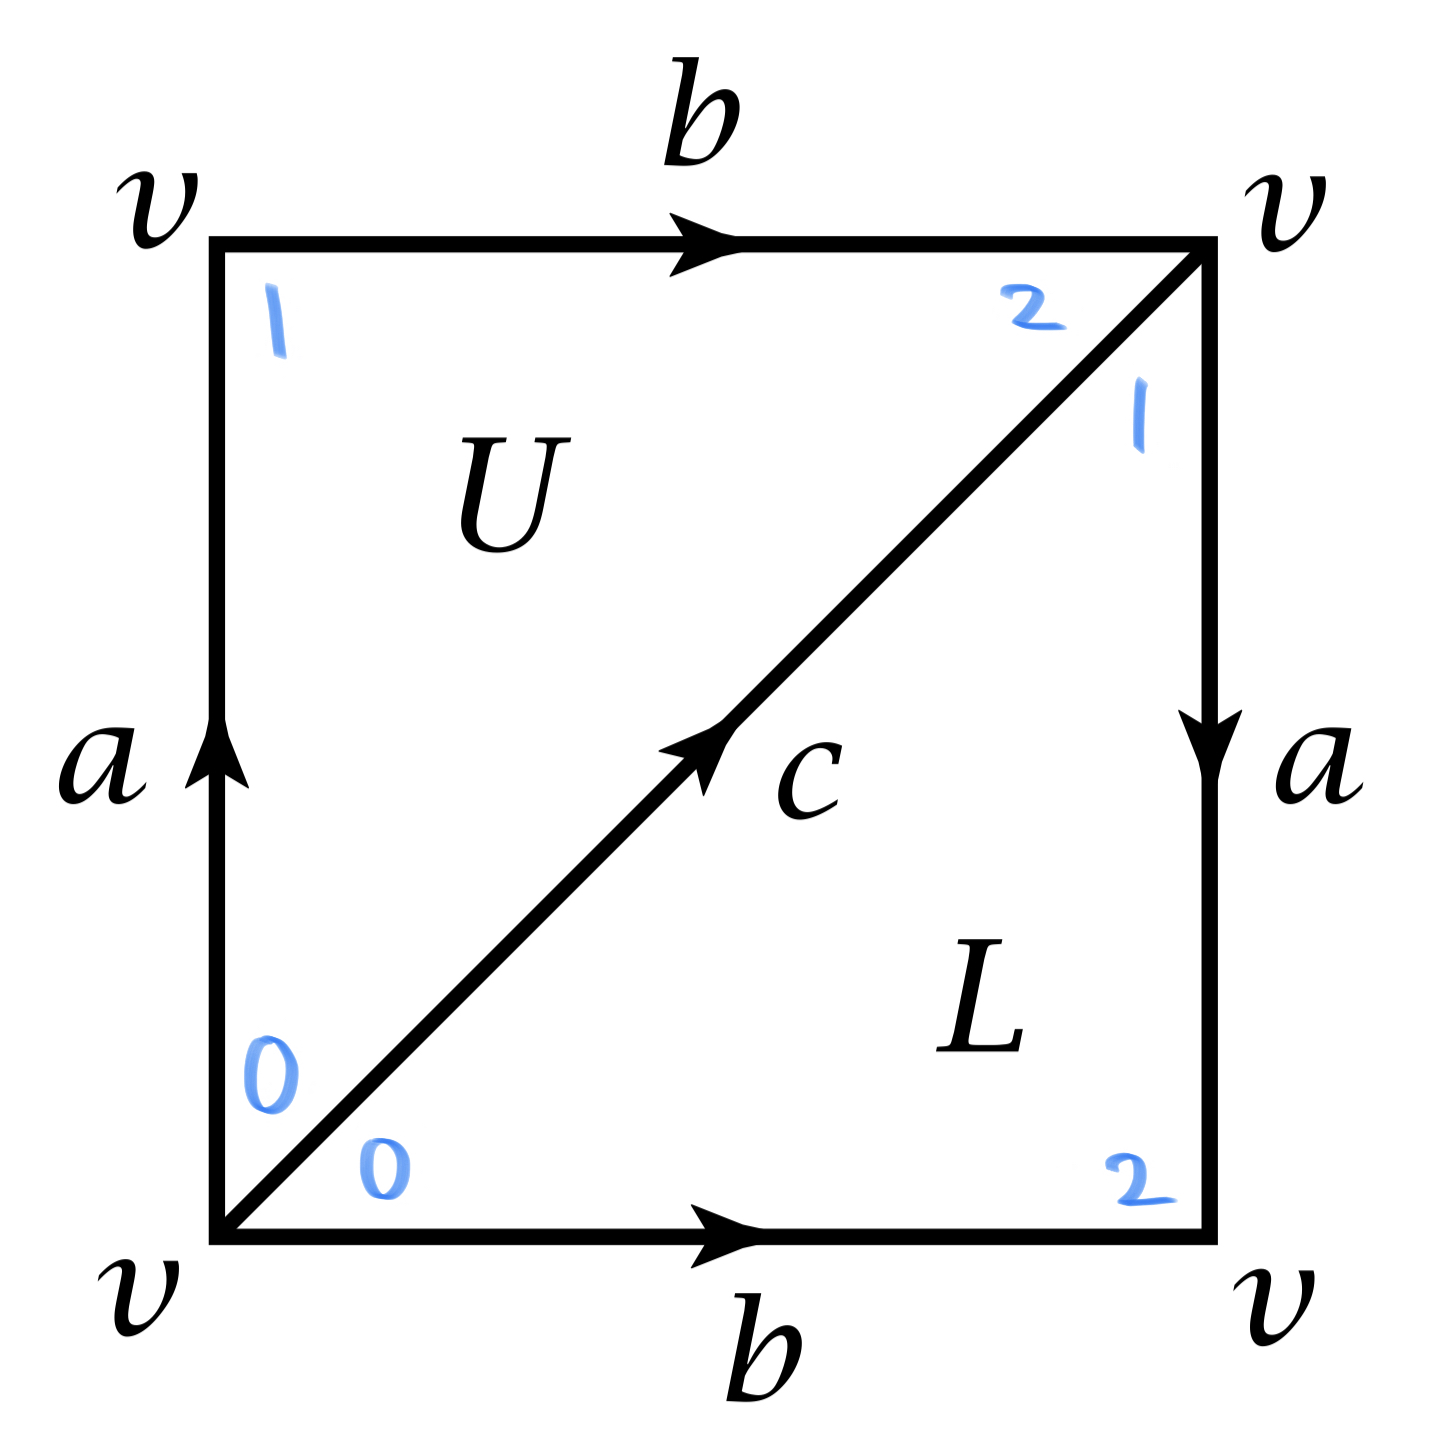
\includegraphics[width=.3\linewidth]{problem5_klein.jpeg}
    \caption{Problem 5}
    \label{fig:problem5_klein}
  \end{figure}

  \begin{align*}
    C_n &= \begin{cases}
      0 & (n \geq 3) \\
      \ev{ U, L } & (n = 2) \\
      \ev{ a, b, c} & (n = 1) \\
      \ev{ v } & (n = 0).
    \end{cases}
  \end{align*}
  $\partial_n = 0$ for $n \geq 3$ and $n = 0$.
  \begin{align*}
    \partial_2(U)
      &= \sum_{i = 0}^2 (-1)^i \sigma \vert [0, 1, 2] \\
      &= \sigma \vert [1, 2] - \sigma \vert [0, 2] + \sigma \vert [0, 1] \\
      &= b - c + a. \\
    \partial_2(L)
      &= \sum_{i = 0}^2 (-1)^i \sigma \vert [0, 1, 2] \\
      &= \sigma \vert [1, 2] - \sigma \vert [0, 2] + \sigma \vert [0, 1] \\
      &= a - b + c.
  \end{align*}

  $\partial_1(a) = 0$ since $\partial_1(a) = \sigma \vert [1] - \sigma \vert [0] = v - v = 0$.
  Similarly, $\partial_1(b) = \partial_1(c) = 0$.
  Thus
  \begin{align*}
    H_n &= \begin{cases}
      \{ 0 \} & (n \geq 3) \\
      \ev{ \sigma } \cong \mathbb{Z} & (n = 2) \\
      \ev{ e_1, e_2, e_3 } \cong \mathbb{Z}^3 & (n = 1) \\
      \ev{ v_0 } \cong \mathbb{Z} & (n = 0).
    \end{cases}
  \end{align*}
  \todo[inline,caption={}]{
    Finish the rest.
  }
\end{proof}

\begin{exer}{(Problem 7)}
  Find a way of identifying pairs of faces of $\Delta^3$ to produce a $\Delta$-complex structure on $S^3$ having a single 3-simplex, and compute the simplicial homology groups of this $\Delta$-complex.
\end{exer}

\begin{exer}{(Problem 8)}
  Construct a 3 dimensional $\Delta$-complex $X$ from $n$ tetrahedra $T_1, \cdots, T_n$ by the following two steps.
  First arrange the tetrahedra in a cyclic pattern as in the figure, so that each $T_i$ shares a common vertical face with its two neighbors $T_{i - 1}$ and $T_{i + 1}$, subscripts being taken mod $n$.
  Then identify the bottom face of $T_i$ with the top face of $T_{i + 1}$ for each $i$.
  Show the simplicial homology groups of $X$ in dimensions 0, 1, 2, 3 are $\mathbb{Z}, \mathbb{Z}_n, 0, \mathbb{Z}$, respectively.
\end{exer}

\begin{proof}
\end{proof}

\end{document}
